\documentclass[a4paper, 10pt, oneside]{book}
\usepackage{float}
\usepackage[utf8]{inputenc}
\usepackage[a4paper,footskip=0.25in]{geometry}
\usepackage{xcolor}
\usepackage{amsmath}
\usepackage{amsthm}
\usepackage{amssymb}
\usepackage{amsfonts}
\usepackage{mathtools}
\usepackage{ dsfont }
\usepackage[most]{tcolorbox}
\usepackage{tikz}
\usepackage{xcolor}
\usepackage{adjustbox}
\usepackage{mathrsfs}
\usepackage{algorithm}
\usepackage{algpseudocode}
\usepackage{marginnote}
\usepackage{xhfill}
\usepackage{mparhack}
\usepackage{pagecolor}
\usepackage{titlesec}
\usepackage{sectsty}
\usepackage{tocloft}
\usepackage{lastpage}
\usepackage{fancyhdr}
\usepackage{tocloft}
\usepackage{hyperref}
\usepackage{etoolbox}
\usepackage{xstring}


\definecolor{mygray}{RGB}{239,240,241}
\definecolor{mycolor}{RGB}{1,50,32}
\usetikzlibrary{babel}
\usetikzlibrary{cd}
\usetikzlibrary{positioning}
\usetikzlibrary{calc}
\usetikzlibrary{arrows.meta}

\geometry{
	left=10mm, % left margin
	textwidth=150mm, % main text block
	marginparsep=5mm, % gutter between main text block and margin notes
	marginparwidth=40mm, % width of margin notes
  bmargin=2cm % height of foot note space
}
\graphicspath{ {./figures/} }
\setlength{\cftchapnumwidth}{2.25cm}
\renewcommand{\cftchappresnum}{\chaptername\ }


\pagestyle{fancy}

\renewcommand{\headrule}{\color{mycolor}\hrulefill}

\newlength\FHoffset
\setlength\FHoffset{1cm}

\addtolength\headwidth{2\FHoffset}

\fancyheadoffset{\FHoffset}

% these lengths will control the headrule trimming to the left and right 
\newlength\FHleft
\newlength\FHright

% here the trimmings are controlled by the user
\setlength\FHleft{1cm}
\setlength\FHright{-3.25cm}

% The new definition of headrule that will take into account the trimming(s)
\newbox\FHline
\setbox\FHline=\hbox{\hsize=\paperwidth%
  \hspace*{\FHleft}%
  \rule{\dimexpr\headwidth-\FHleft-\FHright\relax}{\headrulewidth}\hspace*{\FHright}%
}
\renewcommand\headrule{\color{mycolor}\vskip-.7\baselineskip\copy\FHline}

\renewcommand{\chaptermark}[1]{\markboth{#1}{#1}}
\fancyhead[R]{}
\fancyhead[L]{}
\fancyhead[C]{\hspace{3.25cm}\color{mycolor}\chaptername\ \thechapter\ --\ \leftmark}
\fancyfoot[L]{Page \thepage \hspace{1pt} of \pageref{LastPage}}
\fancyfoot[C]{}

\fancypagestyle{plain}{%
  \fancyhf{}%
  \fancyfoot[L]{Page \thepage \hspace{1pt} of \pageref{LastPage}}
  \renewcommand{\headrulewidth}{0pt}
  \renewcommand{\footrulewidth}{0pt}
  
}

\def\interior{\text{int}}
\def\C{\mathbb{C}}
\def\R{\mathbb{R}}
\def\N{\mathbb{N}}
\def\Q{\mathbb{Q}}
\def\bE{\mathbb{E}}
\def\bP{\mathbb{P}}
\def\Z{\mathbb{Z}}
\def\cA{\mathcal{A}}
\def\cB{\mathcal{B}}
\def\cU{\mathcal{U}}
\def\cC{\mathcal{C}}
\def\cM{\mathcal{M}}
\def\cE{\mathcal{E}}
\def\cF{\mathcal{F}}
\def\cS{\mathcal{S}}
\def\cH{\mathcal{H}}
\def\bH{\mathbb{H}}
\def\cN{\mathcal{N}}
\def\Mloc{\mathcal{M}_{\text{loc}}}
\def\as{\text{ a.s. }}
\def\cov{\text{cov}}
\def\gp{\text{GP}}
\def\tr{\text{tr}}
\def\Id{\text{Id}}
\def\Var{\text{Var}}
\def\EDM{\text{EDM}}
\def\man0{\text{Man}^0}
\def\DM{\text{DM}}
\def\graph{\text{graph}}
\def\Lrw{L_{\text{RW}}}
\def\Lsym{L_{\text{sym}}}
\def\dd{{\text{dd}}}
\def\KL{{\text{KL}}}
\DeclareMathOperator*{\argmin}{\text{argmin}}


\counterwithout*{equation}{equation}
\renewcommand{\theequation}{\arabic{equation}}


\newtheorem{theorem}{Theorem}[chapter]
\newtheorem{corollary}[theorem]{Corollary}
\newtheorem{lemma}[theorem]{Lemma}
\newtheorem{proposition}[theorem]{Proposition}
\newtheorem{definition}[theorem]{Definition}
\newtheorem*{definition*}{Definition}
\newtheorem*{remark}{Remark}
\newtheorem*{aremark}{Added remark}
\newtheorem*{example}{Example}
\newtheorem*{adefinition}{Added definition}
\newtheorem*{example*}{Example}
\newtheorem*{theorem*}{Theorem}
\raggedright


\hypersetup{
    colorlinks=true, %set true if you want colored links
    linktoc=all,     %set to all if you want both sections and subsections linked
    linkcolor=mycolor,  %choose some color if you want links to stand out
    linkbordercolor=mycolor,
    urlcolor=mycolor
}

\titleformat{\chapter}[display]
  {\normalfont\bfseries\flushleft\color{mycolor}}{\Huge\chaptertitlename\ \thechapter:}{0pt}{\Huge}
\sectionfont{\color{mycolor}}
\subsectionfont{\color{mycolor}}


\renewcommand{\cftchapfont}{\color{mycolor}\large\bfseries}
\renewcommand{\cftsecfont}{\color{mycolor}}
\renewcommand{\cftsubsecfont}{\color{mycolor}}
\renewcommand{\cftsubsubsecfont}{\color{mycolor}}

\renewcommand{\cftchapleader}{\color{mycolor}     \cftdotfill{\cftsecdotsep}}
\renewcommand{\cftsecleader}{\color{mycolor}     \cftdotfill{\cftsecdotsep}}
\renewcommand{\cftsubsecleader}{\color{mycolor} \cftdotfill{\cftsecdotsep}}
\renewcommand{\cftsubsubsecleader}{\color{mycolor} \cftdotfill{\cftsecdotsep}}

\def\lecturelist{}
\def\tutlist{}
\newcommand{\beginlecture}[2]{\hypertarget{lec#1}{}\listxadd{\lecturelist}{lec#1}\marginnote{Start of lecture #1 (#2)}}
\newcommand{\begintutorial}[2]{\hypertarget{tut#1}{}\listxadd{\tutlist}{tut#1}\marginnote{Start of tutorial #1 (#2)}}
\newcommand{\dhighlight}[1]{{\color{mycolor}{\underline{{\textbf{#1}}}}}}
\newcommand{\highlight}[1]{{\color{mycolor}{\textbf{#1}}}}
\newcommand{\includeproblem}[2]{
\begin{tcolorbox}[enhanced,breakable,
	title=Problem #1,frame style={color=mycolor}]
	\input{#2}
\end{tcolorbox}}
\newcommand{\includesolution}[2]{
\begin{tcolorbox}[enhanced,breakable,
	title=Solution #1,frame style={color=mycolor}]
	\input{#2}
\end{tcolorbox}}

\renewcommand{\labelitemi}{$\textcolor{mycolor}{\bullet}$}
\renewcommand{\labelitemii}{$\textcolor{mycolor}{\cdot}$}
\renewcommand{\labelitemiii}{$\textcolor{mycolor}{\diamond}$}
\renewcommand{\labelitemiv}{$\textcolor{mycolor}{\ast}$}

\tcolorboxenvironment{corollary}{
  colback=blue!5!white,
  boxrule=0pt,
  boxsep=1pt,
  left=2pt,right=2pt,top=2pt,bottom=2pt,
  oversize=2pt,
  sharp corners,
  before skip=\topsep,
  after skip=\topsep,
  breakable
}

\tcolorboxenvironment{theorem}{
  colback=blue!5!white,
  boxrule=0pt,
  boxsep=1pt,
  left=2pt,right=2pt,top=2pt,bottom=2pt,
  oversize=2pt,
  sharp corners,
  before skip=\topsep,
  after skip=\topsep,
  breakable
}

\tcolorboxenvironment{lemma}{
  colback=blue!5!white,
  boxrule=0pt,
  boxsep=1pt,
  left=2pt,right=2pt,top=2pt,bottom=2pt,
  oversize=2pt,
  sharp corners,
  before skip=\topsep,
  after skip=\topsep,
  breakable
}

\tcolorboxenvironment{proposition}{
  colback=blue!5!white,
  boxrule=0pt,
  boxsep=1pt,
  left=2pt,right=2pt,top=2pt,bottom=2pt,
  oversize=2pt,
  sharp corners,
  before skip=\topsep,
  after skip=\topsep,
  breakable
}

\tcolorboxenvironment{definition*}{
  colback=green!5!white,
  boxrule=0pt,
  boxsep=1pt,
  left=2pt,right=2pt,top=2pt,bottom=2pt,
  oversize=2pt,
  sharp corners,
  before skip=\topsep,
  after skip=\topsep,
  breakable
}

\tcolorboxenvironment{remark}{
  colback=red!5!white,
  boxrule=0pt,
  boxsep=1pt,
  left=2pt,right=2pt,top=2pt,bottom=2pt,
  oversize=2pt,
  sharp corners,
  before skip=\topsep,
  after skip=\topsep,
  breakable
}

\tcolorboxenvironment{aremark}{
  colback=red!5!white,
  boxrule=0pt,
  boxsep=1pt,
  left=2pt,right=2pt,top=2pt,bottom=2pt,
  oversize=2pt,
  sharp corners,
  before skip=\topsep,
  after skip=\topsep,
  breakable
}

\tcolorboxenvironment{example}{
  colback=red!5!white,
  boxrule=0pt,
  boxsep=1pt,
  left=2pt,right=2pt,top=2pt,bottom=2pt,
  oversize=2pt,
  sharp corners,
  before skip=\topsep,
  after skip=\topsep,
  breakable
}

\tcolorboxenvironment{adefinition}{
  colback=blue!5!white,
  boxrule=0pt,
  boxsep=1pt,
  left=2pt,right=2pt,top=2pt,bottom=2pt,
  oversize=2pt,
  sharp corners,
  before skip=\topsep,
  after skip=\topsep,
  breakable
}

\tcolorboxenvironment{aexample}{
  colback=red!5!white,
  boxrule=0pt,
  boxsep=1pt,
  left=2pt,right=2pt,top=2pt,bottom=2pt,
  oversize=2pt,
  sharp corners,
  before skip=\topsep,
  after skip=\topsep,
  breakable
}

\tcolorboxenvironment{definition}{
  colback=green!5!white,
  boxrule=0pt,
  boxsep=1pt,
  left=2pt,right=2pt,top=2pt,bottom=2pt,
  oversize=2pt,
  sharp corners,
  before skip=\topsep,
  after skip=\topsep,
  breakable
}

\tcolorboxenvironment{algorithm}{
  colback=mygray,
  boxrule=0pt,
  boxsep=1pt,
  oversize=2pt,
  left=2pt,right=2pt,top=-12pt,bottom=0pt,
  sharp corners,
  breakable
}

\author{Manuel Hinz}

\addbibresource{Manifolds.bib}

\begin{document}
\newgeometry{left=15mm,right=15mm,bmargin=2cm}
\pagecolor{mycolor}
\begin{titlepage}
    \centering

    \vspace*{1cm}

    % Title and subtitle are enclosed between two rules.
    {\color{white}\rule{\textwidth}{1pt}}

    % Title
    \vspace{.7\baselineskip}
    {\huge {\color{white}\textbf{Lecture notes on Analysis and Geometry on Manifolds}}}

    % Subtitle
    {\color{white}\rule{\textwidth}{1pt}}

    \vspace{1.5cm}

    % Set this size for the remaining titlepage.
    \large

    % Authors side by side, using two minipages as a trick.
    \begin{minipage}{.5\textwidth}
        \color{white}
        \centering
        Written by \\
        Manuel Hinz\\
        {\normalsize mh@mssh.dev or s6mlhinz@uni-bonn.de}
    \end{minipage}%
    \begin{minipage}{.5\textwidth}
        \color{white}
        \centering
        Lecturer\\
        Prof. Dr. Laurent Côté  \\
        {\normalsize lcote[at]math.uni-bonn.de}
    \end{minipage}


    \vspace{3cm}

    % Report logo.
    
\includegraphics[width=.7\textwidth]{Noise_1.0_50.0_32.0}

    \vfill

    % University and date information at the bottom of the titlepage.
    \color{white}{
    University of Bonn \\
    Winter semester 2024/2025\\
    Last update: \today
    }
   
\end{titlepage}
\pagecolor{white}
\tableofcontents

\restoregeometry
\setcounter{chapter}{-1}
\chapter{Manuel's notes}
\begin{tcolorbox}[enhanced,breakable,
	title=Warning,colback=red!20!white]
	These are unofficial lecture notes written by a student. They are messy, will almost surely contain 
    errors, typos and misunderstandings and may not be kept up to date! I do however try my best and use 
    these notes to prepare for my exams. Feel free to email me any corrections to mh@mssh.dev or s6mlhinz@uni-bonn.de.

    Happy learning!
\end{tcolorbox}
\begin{tcolorbox}[enhanced,breakable,
	title=General Information,frame style={color=mycolor}]
    \begin{itemize}
        \item Basis: \href{https://basis.uni-bonn.de/qisserver/rds?state=verpublish\&status=init\&vmfile=no&publishid=252386\&moduleCall=webInfo\&publishConfFile=webInfo&publishSubDir=veranstaltung}{Basis}
        \item Website: \href{https://www.math.uni-bonn.de/~lcote/V3D3\_2024.html}{https://www.math.uni-bonn.de/$\sim$lcote/V3D3\_2024.html}
        \item Time slot(s): \highlight{Tuesday: 14-16} Nussallee Anatomie B and \highlight{Friday: 12-14} GHS
        \item Exams: Tuesday \highlight{11.02.2025, 9-11}, Großer Hörsaal, Wegelerstraße 10 and Friday \highlight{21.03.2025, 9-11}, Großer Hörsaal, Wegelerstraße 10
        \item Deadlines: \highlight{Friday before noon}
    \end{itemize}
\end{tcolorbox}

\section{Organization}

\begin{itemize}\beginlecture{01}{08.10.2024}
    \item Four exercise classes, in the break come to the front and sign up. 
    \item First homework is due this Friday 
    \item Exercise sheets are due on Fridays, every week electronically (groups, at most 2)
    \item No published lecture notes by him!
    \item 5 Minute break right before the full hour
    \item Friday after class for questions
\end{itemize}


\section{Course overview}

He assumes we already know about 
\begin{itemize}
    \item Analysis on \(\R^n\)
    \item Basic point set topology
\end{itemize}

\citation{}
For this class: \dhighlight{smooth manifolds} based on \cite{smooth_manifolds}\marginnote{I would also recommend \cite{differential_geometry}}
\begin{itemize}
    \item Intersection between analysis and topology
    \item Exiting: Connections between those two point of views 
\end{itemize}
\dhighlight{Main topics:}
\begin{enumerate}
    \item[Topic 00:] Topological manifolds 
    \item[Topic 01:] Basic theory of smooth manifolds
    \item[Topic 02:] Vector fields on smooth manifolds
    \item[Topic 03:] Tensor calculus and Stokes' theorem 
    \item[Topic 04:] Lie groups, symplectic and Riemannian geometry     
\end{enumerate}


\chapter{Topological manifolds}

\section{Some point set topology}

Some (set theoretical) conventions for the whole course:
\begin{itemize}
    \item \(A\subset B\) means A subset (not necessarily proper!) of B, i.e. \(\subset =\subseteq\)
    \item A \highlight{neighborhood} of some point \(p\in X\) means \textit{an open set \(U\subset X\) containing \(p\)}
    \item Given \(p=(p_1,\dots,p_n)\in\R^n,r>0\), \(B_r^n(p)\coloneqq \{(x_1,\dots,x_n)\mid \sum_{x_i-p_i}^2<r^2\}\). Often while \(B_s=B_s^n(0)\subset\R^n\)
\end{itemize}

\subsection{Locally Euclidean spaces}

\begin{definition*}
    A topological space \(X\) is called \dhighlight{locally Euclidean of dimension \(n\geq 0\)}, if every 
    point of \(X\) is contained in a neighborhood homeomorphic to some open subset of $\R^n$. 
\end{definition*}

\begin{remark}
    When we speak of a topological space as being \highlight{locally Euclidean}. The dimension is fixed and implicit.
\end{remark}

\begin{definition*}
    Assume that \(X\) is locally Euclidean. A \dhighlight{chart} is a pair \(U,\phi\), where \(U\subset X\),
    \(\phi:U\to\R^n\) is a homeomorphism into its image. Given \(p\in X\), we say that \(U,\phi\) is 
    \dhighlight{centered at \(p\)} if \(p\in U\) and \(\phi(p)=0\in\R^n\)
    \begin{figure}[H]
        \centering
        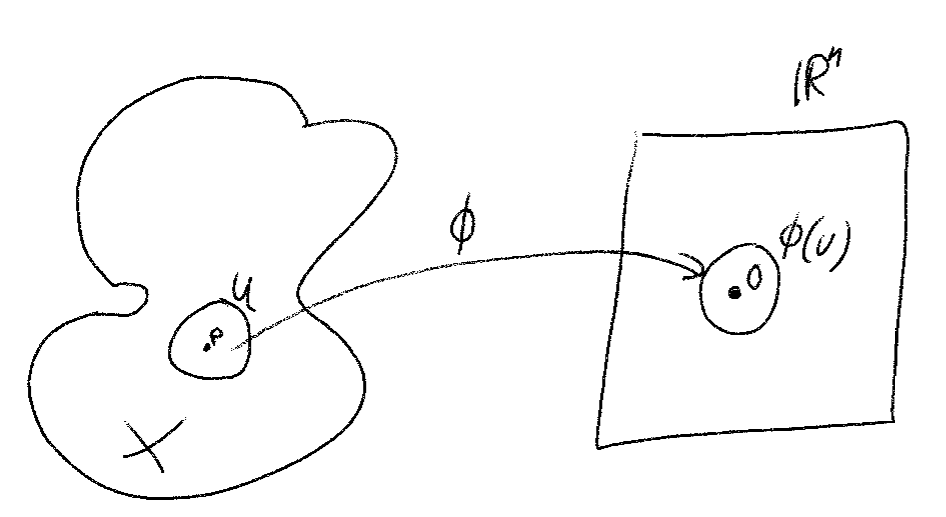
\includegraphics[width=.7\textwidth]{sketch_1_01.png}
        \caption{Sketch 1.01}
    \end{figure}
\end{definition*}

\begin{lemma}\label{lem:1.1}
    The following are equivalent (TFAE):
    \begin{itemize}
        \item \(X\) is locally Euclidean
        \item For any \(p\in X\), there is a chart \(U,\phi\) centered at \(p\) with image \(\phi(U)=B_1\)
        \item For any \(p\in X\), there is a chart \(U,\phi\) centered at \(p\) with image \(\phi(U)=\R^n\)
    \end{itemize}
\end{lemma}

\begin{proof}
    2. and 3. are equivalent, since \(B_1 \simeq \R^n\) are homeomorphic (\(B_1^n\ni x\mapsto \frac{x}{1-\Vert x\Vert}\))
    
    2. \(\implies \) 1. is tautological

    1. \(\implies\) 2. given \(p\in X\), since \(X\) is locally Euclidean, there exists \highlight{some} chart \(U,\phi\), \(p\in U\).
    \(psi:U\to\R^n\), homeo onto its image \(psi(U)=O\subset\R^n\). By translativity \(\R^n\ni x\mapsto x-\psi(p)\), one can assume 
    \(\psi(p)=0\in\R^n\). By scaling \(\R^n (x\mapsto \lambda x,\lambda>0)\), can assume \(B_1\subset\psi(U)\).
    Let \(U'=\psi^{-1}(B_1)\), then \((U,\psi)\) as claimed. 
\end{proof}

\subsection{Hausdorff spaces}

\begin{definition*}
    A topological space \(X\) is called Hausdorff, if given any \(p_1\neq p_2\),\(p_1,p_2\in X\), there exist neighborhoods \(p_1\in U_1,p_2\in U_2\) s.t. \(U_1\cap U_2=\emptyset\).
  \begin{figure}[H]
        \centering
        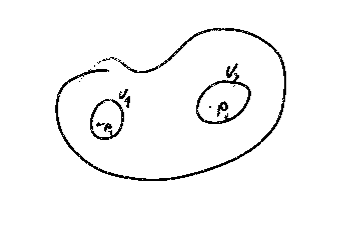
\includegraphics[width=.7\textwidth]{sketch_1_02.png}
        \caption{Sketch 1.02}
    \end{figure}
\end{definition*}

\begin{example}
    \begin{itemize}
        \item \(\R^n\)
        \item CW complexes
        \item most reasonable spaces
    \end{itemize}
\end{example}

\begin{example}[Not Hausdorff]
    \(X=\{0,1\}\), open subsets \(\emptyset,\{0\},\{0,1\}\)
\end{example}

\begin{remark}
    \(X\) is homeomorphic to \(\R/\R^*\) (quotient topology), \(R^*, (s,x\mapsto sx)\)
\end{remark}


\begin{lemma}\label{lem:1.2}
    Let \(X\) be Hausdorff. 
    \begin{enumerate}
        \item[(a)] point sets \(\{x\}\) are closed
        \item[(b)] convergent sequences have unique limits. (\(x_n\to p,x_n\to q\implies p=q\)) 
        \item[(c)] compact sets are closed 
    \end{enumerate}
\end{lemma}

\begin{proof}
    (c) \(\implies \) (a)

    For (c): Let \(K\subset X\) be compact. Want to show \(K^c\) is open. Pick \(p\in K^c\). For each 
    \(q\in K\), we can choose \(U_q\ni q, U_p\ni p: U_q\cap U_p=\emptyset\) Since K is compact, it can be covered by \(U_{q_1},\dots,U_{q_l}\). Then \(\bigcap_{i=1}^l U_{q_i}\) is oen and contains 
    \(p\), disjoint, then \(\bigcup_{i=1}^l U_{q_i}\supset K\).

    \begin{figure}[H]
        \centering
        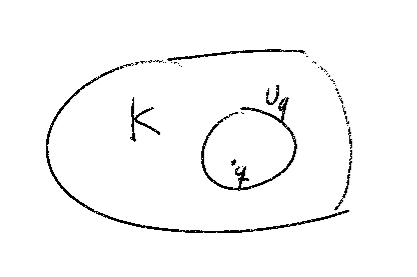
\includegraphics[width=.7\textwidth]{sketch_1_03.png}
        \caption{Sketch 1.03}
    \end{figure}

    (b) Suppose for contradiction that \(x_i\to p,x_i\to q\) and \(p\neq q\). Since \(X\) is Hausdorff, \(\exists U\ni p, O\ni q, U\cap O=\emptyset\). But for \(N>>0 x_i\in U, x_i\in O\forall i>N\)
\end{proof}


\subsection{Basis and covers}

Let \(X\) be a topological space.

\begin{definition*}
    A collection \(\cB\) of subsets of \(X\) is called a \dhighlight{basis(base)} for \(X\), if for any \(p\in X\)
    and any neighborhood \(U\ni p\), there exists an element \(\cU\in\cB\) s.t. \(p\in \cU\subset U\).
    \begin{figure}[H]
        \centering
        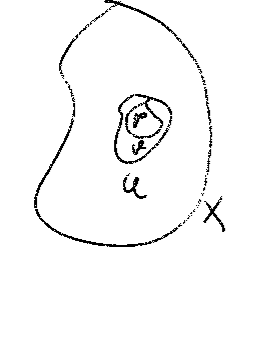
\includegraphics[width=.7\textwidth]{sketch_1_04.png}
        \caption{Sketch 1.04}
    \end{figure}
\end{definition*}


\begin{lemma}\label{lem:1.3}
    \(\cB\) is a basis for \(X\iff\) every open set of \(X\) is a union of elements of \(\cB\).
\end{lemma}

\begin{proof}
    Trivial.
\end{proof}

\begin{definition*}
    A topological space \(X\) is \dhighlight{second-countable} if it admits a countable basis.
\end{definition*}

\begin{example}
    \begin{itemize}
        \item \(\R^n\), \(\cB=\{B_s^n(p)\mid s\in \Q_+,p=(p_1,\dots,p_n)\in\Q^n\subset \R^n\}\)
    \end{itemize}
\end{example}

\begin{lemma}\label{lem:1.4}
    The property of being second-countable is closed under 
    \begin{enumerate}
        \item[(a)] subspaces
        \item[(b)] countable disjoint unions
        \item[(c)] countable products
    \end{enumerate}
\end{lemma}

\begin{remark}
    The property of being second-countable is not closed under arbitrary quotients \(q:A\to A/B\). 
    An obvious sufficient conditions is for \(q\) to be an open map. (Since it is a pushforward)\marginnote{When constructing manifolds via quotients, check that it is still second-coutable!}
\end{remark}

\begin{lemma}\label{lem:1.5}
    If \(X\) is second countable, then any open cover of \(X\) admits a countable subcover.
\end{lemma}

\begin{proof}
    Let \(\cB\) be a countable basis for \(X\). Let \(\cC\) be an open cover. 
    Let \(\tilde{\cB}\subset\cB\) be the collection of basis elements \(U\), which are contained 
    in some \(\cU\in\cC\). Observe (key!) \(\tilde{\cB}\) is a cover of \(X\). For each \(U\in\tilde{\cB}\),
    choose \(\cU_U\in\cC\) such that \(U\subset \cU_U\). Then \(\{\cU_U\}\) is a countable subcover of \(\cC\).
\end{proof}

\begin{definition*}
    Let \(X\) be a topological space. An \dhighlight{exhaustion of \(X\) by compact subsets} is a sequence \(\{K_i\}_{i\in\N}\),
    where \(K_i\subset X\) compact and \(K_i\subset \interior(K_{i+1})\) and \(\bigcup_{i=1}^\infty K_i=X\).
\end{definition*}

Recall given \(A\subset X\). \(\interior(A)\coloneqq \{x\in A\mid x \text{ in a neighborhood } U\subset A\}\).


\begin{lemma}\label{lem:1.6}
    If \(X\) is locally Euclidean, Hausdorff\footnote{not needed} and second countable. Then \(X\) admits an exhaustion by compact subsets.
\end{lemma}

\begin{proof}
    Since \(X\) is locally Euclidean, admits a basis \(\cB\) of open subsets having compact closure.\marginnote{That is take the close of \(B_{\frac{1}{2}}\subset\R^n\)}
    \begin{figure}[H]
        \centering
        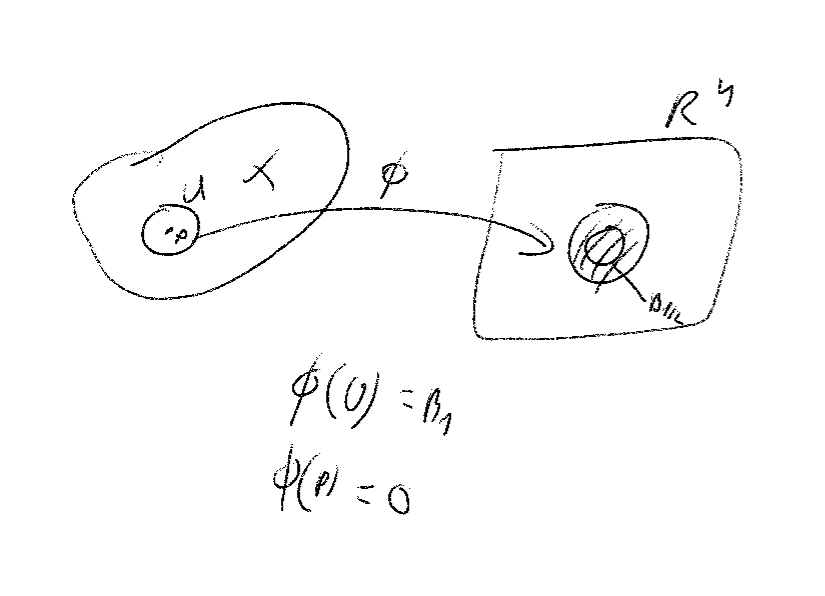
\includegraphics[width=.7\textwidth]{sketch_1_05.png}
        \caption{Sketch 1.05}
    \end{figure}
    By Lemma 1.5, one can extract a countable subcover \(\{U_i\}_{i=1}^\infty\). Set \(K_1=\overline{U_1}\).
    Assume that we already constructed \(K_1,\dots,K_k\) such that \(U_j\subset K_j\)
    and \(K_{j-1}\subset\interior(K_j),j\geq 2\). Since \(K_k\) is compact and \(K_k\subset X=\bigcup_{i=1}^\infty U_i\), then there exists some \(m_k\) such that 
    \(K_k\subset X=\bigcup_{i=1}^{m_k} U_i\) by compactness. Might as well assume that \(m_k\geq k\). Set 
    \[K_{k+1}=\overline{\bigcup_{i=1}^{m_k} U_i}=\bigcup_{i=1}^{m_k} \overline{U_i}.\] By construction \(K_{k+1}\) 
    is compact, \(K_k\subset \interior(K_{k+1})\). We get \(\{K_j\}_{j=1}^\infty\), \(U_j\subset K_j\) (because \(m_j\geq j\)) \(\implies \bigcup_{i=1}^\infty U_i=\bigcup_{i=1}^\infty K_i\)
\end{proof}
\beginlecture{02}{11.10.2024}

\begin{definition*}\label{def:local_finiteness}
    Let \(X\) be a topological space. Let \(\cC\) be a collection of subsets of \(X\). We say that \(\cC\) 
    is \dhighlight{locally finite} if for every \(x\in X\) there exists a neighborhood \(U\ni x\) such that 
    the intersection of \(U\) with all but finitely many elements of \(\cC\) is empty.
\end{definition*}

\begin{example}[Example for local finiteness]
    Take \(X=\R\), \(\cC=\{(i-1,i+1)\}_{i\in\Z}\).
    \begin{figure}[H]
        \centering
        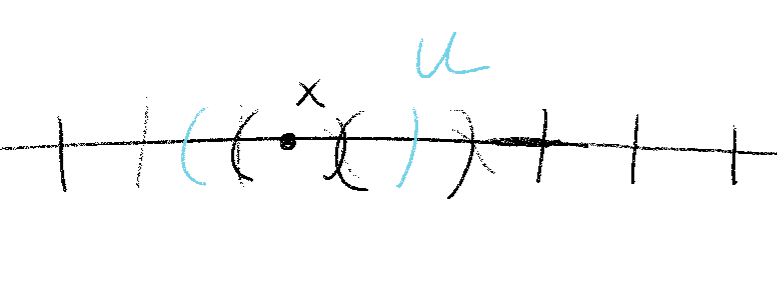
\includegraphics[width=.7\textwidth]{sketch_1_06.png}
        \caption{Sketch 1.06}
    \end{figure}
\end{example}

\begin{example}[Non-example for local finiteness]
    \(X=\R\), \(\cC=(q-1,q+1)_{q\in\Q}\)
\end{example}

\begin{definition*}\label{def:refinement}
    Let \(X\) be a topological space. Let \(\cC\) be a cover of \(X\). A cover \(\cC'\) of \(X\) is called a 
    \dhighlight{refinement of \(\cC\)}, if for all elements \(U\in\cC'\), there exists such \(V\in\cC\): \(U\subset V\).
\end{definition*}

\begin{example}[Example of Refinement]
   In the proof of lemma \ref{lem:1.5}, we showed that any open cover admits a refinement by basis elements. 
\end{example}

\begin{definition*}
    A topological space \(X\) is called \dhighlight{paracompact} if every open cover admits a locally finite refinement.
\end{definition*}

Whats up with the word \highlight{para}compact? It's like compact, but weaker! It is necessary that it only admits a locally finite refinement!

\begin{lemma}\label{lem:1.7}
    Let \(X\) be Hausdorff and suppose that \(X\) admits an exhaustion by compact subsets. Then 
    \(X\) is paracompact.In fact, we will show that given any basis \(\cB\) of \(X\), any open cover 
    admits a locally finite refinement by elements of \(\cB\).
\end{lemma}

\begin{proof}
    By assumption, \(\{K_i\}_{i\in \N}\), \(K_i\) compact, \(K_i\subset\interior(K_{i+1}),\bigcup_{i=1}^\infty K_i=X\).\marginnote{Careful! There are many definitions of exhaustion by compact sets \dots}
    Let, for  \(j\in\Z: V_j=K_{j+1}\setminus \int (K_j)\) if \(j\leq 0: K_j=\emptyset\)\footnote{He writes \(-\) for \(\setminus\)}.
    \begin{figure}[H]
        \centering
        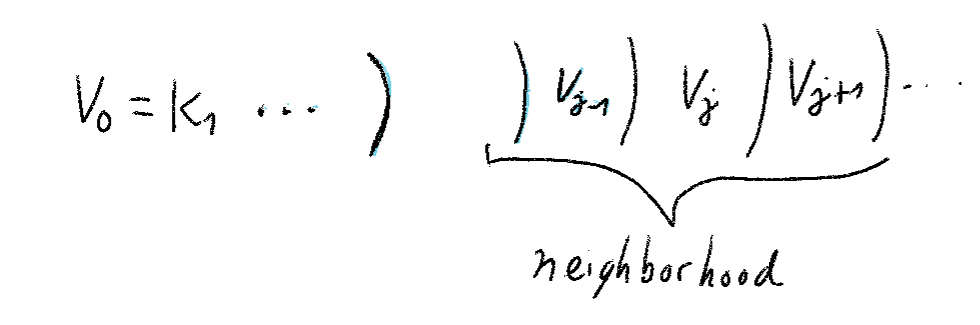
\includegraphics[width=.7\textwidth]{sketch_1_07.png}
        \caption{Sketch 1.07}
    \end{figure}
    Notice:
    \begin{itemize}
        \item \(V_j\) is compact, since we take the intersection of a compact set and a closed set. (\(\interior(K_j)^c\) is closed)
        \item \(\bigcup_{j\in \Z} V_J=X\), since \(\bigcup_{j\leq n}=\bigcup_{j\leq n+1} K_j=K_{j+1}\)
        \item The compact sets \(V_j\) are intersecting (along their boundary?) \(V_j\cap V_{j-1}=\partial K_j\coloneqq K_j\setminus\interior(K_j)\)
    \end{itemize}
    Evidently \marginnote{Here we use Hausdorffness}\(\{U_\alpha \cap \interior(K_{j+1})\cap \interior(K_{j-1})^c\}_{\alpha\in\cA}\) covers \(V_j=K_{j+1}-\setminus K_{j-1}^c\), where the \(\{U_\alpha\}_{\alpha\in\cA}\) is an open cover.
    Since \(\cB\) is a basis, we can find a refinement of this cover by basis elements. Since \(V_j\) are compact, we can extract a 
    finite subcover \(\{V_l^j\}_{l=1,\dots,k_j}\). Let's consider: \(\{V_l^j\}_{j\in Z, l=1,\dots,k_j}\). This 
    subcover works, i.e. 
    \begin{itemize}
        \item obviously a cover, since the \(V_j\) cover \(X\), obviously a refinement of \(\{U_\alpha\}\) 
        \item locally finite: given \(x\in X, x\in V_j\), hence \(x\in \interior(K_{K_{j+2}})\cap K_{j-1}^c\eqqcolon U\). If 
              \(U\cap V_l^k\), then we must have \(j-2\leq k\leq j+2\). But \(\{V_l^k\}_{j-2\leq k\leq j+2}\) is finite. \qedhere  
    \end{itemize} 
\end{proof}

\begin{corollary}\label{cor:1.8}
    If \(X\) is locally Euclidean, Hausdorff and second countable \(\implies X\) is paracompact.
\end{corollary}

\begin{proof}
    By lemma \ref{lem:1.6} (exhaustion by compact subsets) and lemma \ref{lem:1.7} \(\implies\) paracompact.
\end{proof}
\begin{customclr}{1.8'}\label{cor:1.8'}
    Let \(X\) be Euclidean amd Hausdorff. Then \(X\) is second countable iff \(X\) has countably many components and \(X\) is paracompact.
\end{customclr}
\begin{remark}
    There are different definitions of manifolds. They differ in either forcing second countability or paracompactness. This lemma shows 
    that there only is a difference if there are uncountably many components.
\end{remark}

\begin{proof}
    Corollary \ref{cor:1.8} and the bonus homework problem from sheet 01.
\end{proof}

\begin{remark}
    Basis elements are open.
\end{remark}

\section{Topological manifolds}

\begin{definition*}
    A \dhighlight{topological \(n\)-manifold} \(M\) is a topological space with the following properties:
    \begin{enumerate}
        \item[(i)]   \(M\) is locally Euclidean (of dimension \(n\)) 
        \item[(ii)]  \(M\) is Hausdorff
        \item[(iii)] \(M\) is second countable 
    \end{enumerate}
\end{definition*}    

Morally we only really need condition (i). Why do we need the others? 
For (ii) you will not get a useful theory without it, while (iii) can be replaced by paracompactness (see corollary \ref{cor:1.8'}).

\begin{definition*}
    Let Man$^0$ be the category of topological manifolds with 
    \begin{enumerate}
        \item objects: topological manifolds 
        \item morphisms: continuous functions  
    \end{enumerate}
\end{definition*}

\begin{remark}
    \(\man0\) full subcategory of Top.
\end{remark}

\begin{remark}
    By definition, \(M,N\in\man0\), then \(M,N\) are isomorphic iff \(M,N\) are homeomorphic.
\end{remark}

\subsection{Examples of topological manifolds}

\begin{example}[Spaces isomorphic to \(R^n\)]
    \(\R^n,n\geq 0\) More generally, if \(V\) a finite dimensional \(\R\)-vector space, then \(V\)
    is a topological \(n\)-manifold.
\end{example}

\begin{example}
    Any open subset of \(\R^n\)
\end{example}

\begin{example}[Graphs]
    Let \(U\subseteq \R^n\) open, let \(f:U\to\R^n\) be a continuous function. We set 
    \[M\coloneqq\text{graph}(f)\coloneqq \{(x,y)\in U\times \R^n\mid y=f(x)\}.\]
    Then \(M\) is a manifold. The map \(M\to U\) by \((x,y)\mapsto U\) gives a global chart.
\end{example}

\begin{example}[Spheres]
    Let \(S^n\coloneqq \{x_0^2+\dots+x_n^2=1\}\subset \R^{n+1}\). Then \(S^n\) is a manifold\marginnote{Here we no longer have a global chart (for topological reasons)}.
    We define charts \[\phi_i^{\pm}:U_i^\pm = \{(x_0,\dots,x_n)\in S^n\mid \pm x_i>0\}\to B_1^n(0)\]
    by \((x_0,\dots,x_n)\mapsto (x_0,\dots,\hat{x}_i,\dots,x_n)\coloneqq (x_0,\dots,x_{i-1},x_{i+1},\dots,x_n)\)
    \begin{figure}[H]
        \centering
        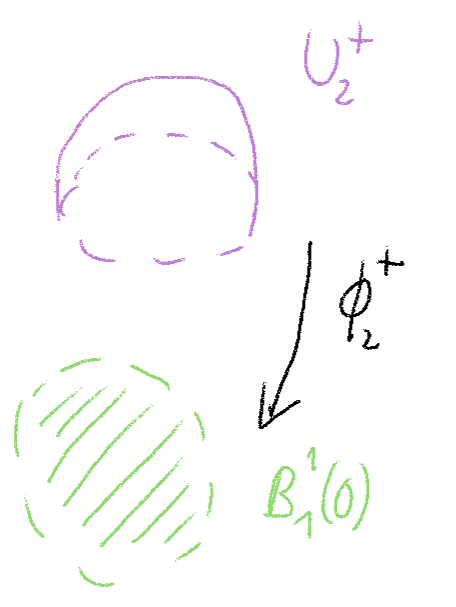
\includegraphics[width=.7\textwidth]{sketch_1_08.png}
        \caption{Sketch 1.08}
    \end{figure}
\end{example}

\begin{example}[spheres']
    Let \(C^n\coloneqq \partial([-1,1]^{n+1})=[-1,1]^{n+1}\setminus\interior([-1,1]^{n+1})\).
    Homework: \(C^n\simeq S^n\) (homeomorphic)
\end{example}

\begin{example}[\(n\)-torus]
    Let \(\Pi^n\coloneqq \R^n/\Z^n\) with the quotient topology. Then this is a manifold (exercise).
    \begin{figure}[H]
        \centering
        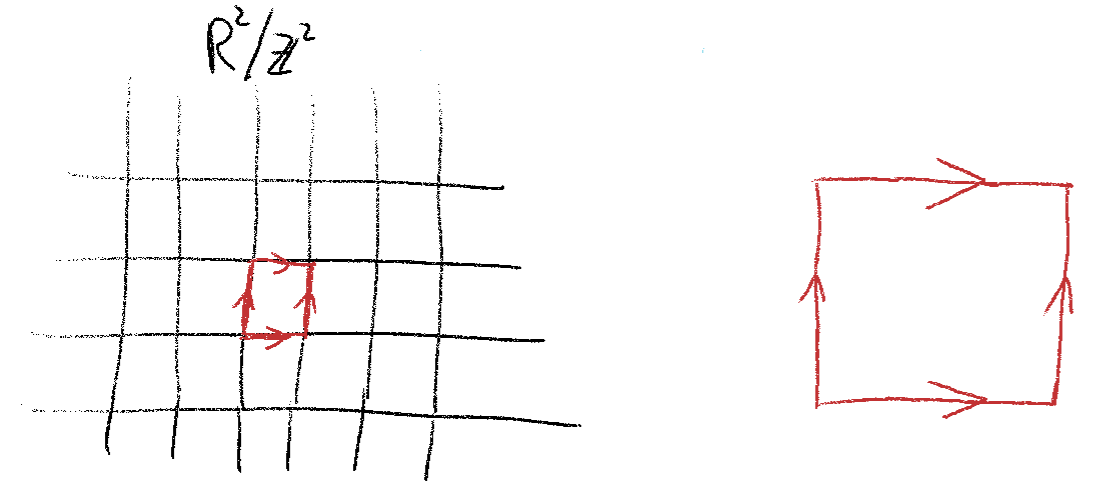
\includegraphics[width=.7\textwidth]{sketch_1_09.png}
        \caption{Sketch 1.09}
    \end{figure}
\end{example}

\begin{example}[\(\R\bP^n\coloneqq S^n/\{x\sim -x\}\)]
    \(\R\bP^n\) are also manifolds (called the real projective spaces).
\end{example}

\begin{example}[Klein bottle]
    \begin{figure}[H]
        \centering
        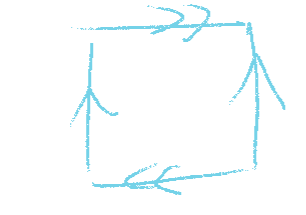
\includegraphics[width=.7\textwidth]{sketch_1_10.png}
        \caption{Sketch 1.10}
    \end{figure}
\end{example}

\begin{remark}
    \(\R\bP^2\) or generally \(\R\bP^{2n}\) and the Klein bottle are not orientable.
\end{remark}

\subsection{Brief interlude: Why do we need Hausdorffness?}

\begin{itemize}
    \item Back in the day (Riemann) 
    \item There is no hope to classify even 1d locally Euclidean, second-countable NOT Hausdorff spaces (See the line with two origins)
    \item With Hausdorff: Only 1d manifolds are \(\R,S^1\) (see website) 
\end{itemize}
Why do we need second countability? 
\begin{itemize}
    \item Subspaces of \(\R^n\) are second countable 
    \item We want partitions of unity (paracompactness suffices for that)
\end{itemize}

\subsection{Manifolds with boundary}

Let \(\bH^n\coloneqq \{(x_1,\dots,x_n)\in\R^n\mid x_n\geq 0\}\).
\begin{definition*}
    A \dhighlight{manifold with boundary} is a topological space with the following properties:
    \begin{enumerate}
        \item[(i)] Every point has a neighborhood homeomorphic to an open subset of \(\bH^n\)
        \item[(ii)] Hausdorff
        \item[(iii)] second countable   
    \end{enumerate}
\end{definition*}

Clearly every manifold is also a manifold with boundary.

\begin{example}
    \(\bH^n\) is a manifold with boundary, but not a manifold. Since for points on the boundary, there are no neighborhoods homeomorphic to Euclidean space.
\end{example}

\begin{example}
    \(S^n\cap \cH^{n+1},S^n\subset\R^{n+1}\), \([a,b],[0,\infty)\)
    \begin{figure}[H]
        \centering
        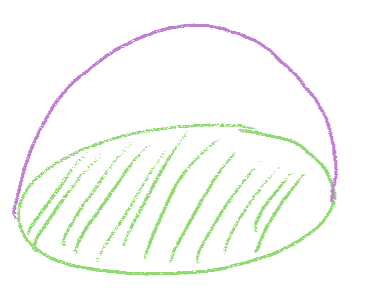
\includegraphics[width=.7\textwidth]{sketch_1_12.png}
        \caption{Sketch 1.12}
    \end{figure}
\end{example}

\begin{definition*}
    If \(M\) manifold with boundary, we say \(x\) is a \dhighlight{boundary point}, if \(x\in M\setminus\interior(M)\) (i.e. it has no neighborhood homeomorphic to Euclidean space?), otherwise \(x\) is an iterior point. We let \(\partial M \coloneqq \{\text{boundary points}\}\).
\end{definition*}

\beginlecture{03}{15.10.2024} 

\dhighlight{Addendum to the last lecture:}

\begin{remark}
    Most of what he says in the course can be generalized to manifolds with boundary (unless it makes no sense).
    Those results are only stated (and proofed) for manifolds. it might be a good exercise to go through the notes and generalize the statements to manifolds with boundary.
\end{remark}

\subsection{Elementary topological properties of topological manifolds}

\marginnote{Not proved here, but we are welcome to use}

\begin{itemize}
    \item A manifold is connected iff it is path connected 
    \item For manifolds, all forms of compactness (ordinary compactness (every open cover has a finite subcover), limit point compactness, sequential compactness) are equivalent
    \item All manifolds are metrizable (Urysohn metrization theorem + second countable \(\implies\) metrizable) 
    \marginnote{The first two point were proven on the first sheet. The last two use countability}    
    \item Any manifold is homotopy equivalent to a countable CW complex (Milner?) \(\pi_k(M)\) are countable
\end{itemize}

\section{Classification of topological manifolds (proofs are not examinable)}
\subsection{Classification of 1-dimensional manifolds}
\begin{theorem}\label{thm:1.9}
    Any connected one dimensional manifold is homeomorphic to  
    \begin{itemize}
        \item \(\R^1\) or
        \item \(\bH^1\)
    \end{itemize}
\end{theorem}

\begin{proof}
    See Course website: \cite{gale_classification_takehome} in the form of a take-home exam
\end{proof}

\begin{remark}
    If you allow a boundary, then you also have \([0,1],[0,1)\). 
\end{remark}

\subsection{Classification of 2-dimensional manifolds}
\marginnote{2-dimensional manifolds are often called surfaces}
\begin{itemize}
    \item \(S^2=\{(x_0,x_1,x_2)\in\R^3\mid \sum_{i=0}^2 x_i^2=1\}\)
    \item \(\Pi^2 \coloneqq \R^2/\Z^2\)
    \item \(\R\bP^2=S^2/\{x\sim -x\}\)
\end{itemize}

\dhighlight{Construction}(Connected sum of surfaces):
\begin{figure}[H]
    \centering
    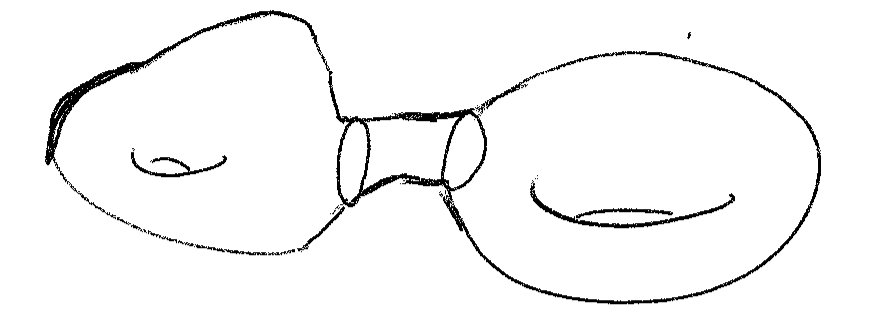
\includegraphics[width=.7\textwidth]{sketch_1_14.png}
    \caption{Sketch 1.14}
\end{figure}
Let \(M_1,M_2\) be surfaces (i.e. 2-dimensional manifolds). Choose charts \(M_i\supset U_i\stackrel{\phi_i}{\to} B_1\subset \R^2\).
Let \(\acirc{M}_i = M_i \setminus \phi_i^{-1}(B_{\frac{1}{2}})\). Let \(M_1 \# M_2 \coloneqq \acirc{M}_1 \perp \acirc{M}_2 /\sim\),
where \(X\in \acirc{M}_1 \sim y\in \acirc{M}_2\) if \(x\in \phi_1^{-1}(\partial \overline{B_{\frac{1}{2}}})\) and \(y=(\phi_2^{-1}\circ \phi_1) (x)\)

\dhighlight{Facts:}
\begin{itemize}
    \item If \(M_1,M_2\) are connected, then \(M_1\# M_2\) is well defined up to 
    homeomorphism.
    \item The operation of connected sum is also well defined for connected \(n\)-manifolds 
    \item (for the future) The operation of connected sum also works in the smooth category.
\end{itemize} 

\begin{theorem}[Classification of surfaces]\label{thm:1.10}
    Every compact, connected surface is homeomorphic to one of the following manifolds:
    \begin{itemize}
        \item \(S^2\)
        \item \(\underbrace{\Pi^2\# \dots \# \Pi^2}_{k\text{ times}}\)
        \item \(\underbrace{\R\bP^2\# \dots \# \R\bP^2}_{l\text{ times}}\) (non-orientable)
    \end{itemize}
    \begin{figure}[H]
        \centering
        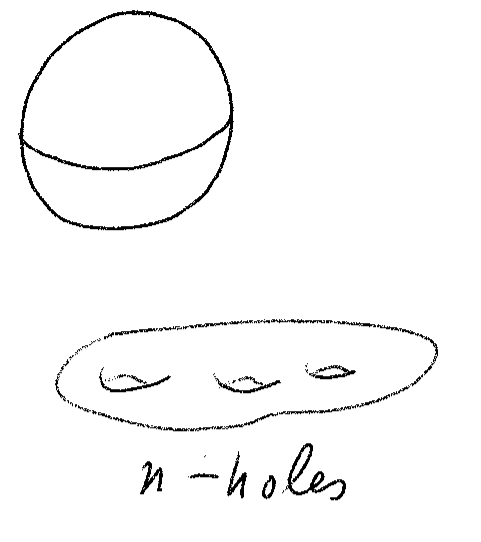
\includegraphics[width=.4\textwidth]{sketch_1_15.png}
        \caption{Sketch 1.15}
    \end{figure}
\end{theorem}

\begin{remark}
    Surfaces are classified by the following invariants:
    \begin{enumerate}
        \item[(a)] orientability
        \item[(b)] Euler characteristic   
    \end{enumerate}
    For later: This classification also works in the smooth category.
\end{remark}

\subsection{Classification of high dimensional manifolds (not examinable at all)}

\dhighlight{Poincaré conjecture} (now theorem of G. Perelman (2003), W. Thurston (1980s)):
Any compact connected \(3\) dimensional manifold which is \dhighlight{simply connected }
is homeomorphic to \(S^3\). This paper is all about PDEs and Ricci flows. 

\dhighlight{Generalized Poincaré conjecture}: Any \(n\)-manifold, which is homotopy equivalent to \(S^n\) 
is homeomorphic to \(S^n\). This is true in all dimensions. for \(n\geq 5\) Smale in the 1960s,
for \(n=4\) Freedsen in the 1980s.

Unlike in dimension 1,2,3 the classification of \(n\geq 3\)-dimensional manifolds is 
complicated and not complete.

\begin{example}
    Any finitely presented group arises as the fundamental group of a compact 
    connected \(4\)-manifold(Which is provably too hard). 
\end{example}








\chapter{Smooth manifolds}
\section{Basic theory}
\subsection{Charts and atlases}
\begin{definition*}
    Given \(U\subset\R^n\) open, a function \(f:U\to \R^m, f=(f_1,\dots,f_m)\) is called 
    \dhighlight{smooth} (or \dhighlight{\(\C^\infty\)} or \dhighlight{infinitely differentiable}), if the 
    \dhighlight{component functions} \(f_i\) admit all partial derivatives of all orders and all these partial derivatives are continuous.
\end{definition*}
In other words \(f\) smooth: \(\iff\forall 1\leq i\leq m,\alpha=(\alpha_1,\dots,\alpha_n)\in\N^n,\partial_{\alpha} f\coloneqq \partial_{x_1}^{\alpha_1} \dots \partial_{x_n}^{\alpha_n} f\) exists.

\begin{remark}
    Given \(k\geq 0\), we can similarly say hat \(f\) is \dhighlight{\(k\)-times continuously differentiable} and write \((f\in)\) and write \(f\in C^k(U,\R^m)\), if 
    for all \(\alpha=(\alpha_1,\dots,\alpha_n)\in\N^n,\sum\alpha_i \leq k\) \(\partial_x^\alpha f_i\) is continuous for all \(i\).
\end{remark}

\begin{definition*}
    Let \(M\) be a topological manifold. We say that two charts \((U_1,\phi_1)\), \((U_2,\phi_2)\)
    are \dhighlight{smoothly compatible} if the map \(\phi_2\circ \phi_1^{-1}:\phi_1(U_1\cap U_2)\to\phi_2(U_1\cap U_2)\)
    is smooth. We call \(\phi_2\circ\phi_1^{-1}\) a \dhighlight{transition function}.
    \begin{figure}[H]
        \centering
        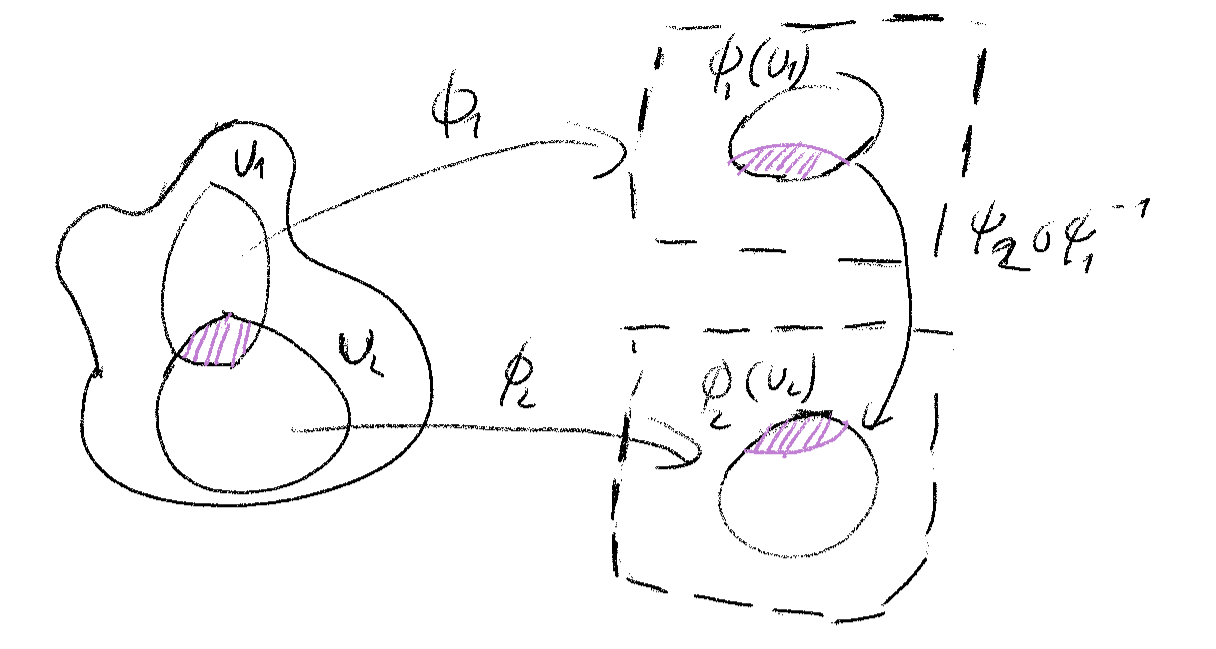
\includegraphics[width=.7\textwidth]{sketch_2_01.png}
        \caption{Sketch 2.01}
    \end{figure}
\end{definition*}

\begin{definition*}
    Let \(M\) be a topological manifold. An \dhighlight{(smooth) atlas} \(\cA\) of \(M\) is a collection of charts 
    \(\{U_\alpha,\phi_\alpha\}_{\alpha\in\cA}\) such that 
    \begin{itemize}
        \item the \(\{U_\alpha\}\) cover \(M\)
        \item the charts are pairwise smoothly compatible (i.e. for all \(\alpha,\beta\in\cA (U_\alpha,\phi_\alpha),(U_\beta,\phi_\beta)\) are smoothly compatible).
    \end{itemize}
\end{definition*}

\begin{definition*}
    We say that two atlases \(\cA,\cA'\) (on a fixed topological manifold) are \dhighlight{equivalent}, if their union 
    \(\cA\cup\cA'\) is still an atlas.
\end{definition*}

\dhighlight{Fact(Sheet 03):}
This defines an equivalence relation.

\begin{definition*}
    A \dhighlight{smooth manifold} \(M=(M,[\cA])\) consists of the following data:
    \begin{enumerate}
        \item[(i)] a topological manifolds \(M\)
        \item[(ii)] an equivalence class of smooth atlases 
    \end{enumerate}
\end{definition*}


\begin{remark}
    \begin{itemize}
        \item typically, we will designate smooth manifolds by a capital letter, e.g. \(M\). But we always mean \((M,[\cA])\).
              \dhighlight{Note} being a smooth manifolds is \dhighlight{extra} structure on a topological space, while being a topological manifold is a property
        \item Using Zorn's lemma, it can be shown that any atlas is contained in a \dhighlight{unique maximal atlas}. Uniqueness here does not use Zorn's lemma, only existence needs that! Equally well define a smooth manifold to 
              be a topological manifold and a maximal atlas.\marginnote{Typically we are given an atlas, since the maximal atlases have uncountably mani charts, which is why we work with equivalence classes, rather than maximal atlases}
        \item \(\forall 0\leq k\leq \infty\), we can define the notion of a \(C^k\)-atlas, simply by requiring that the transition functions are 
              \(C^k\) functions. This yields the definition of \(C^k\)-Manifolds. Two extreme cases: \(C^0\)-manifold (topological manifolds) and \(C^\infty\)-manifolds. Any \(k\geq 1\) is not more interesting than \(C^\infty\)!
    \end{itemize}
\end{remark}

\beginlecture{04}{18.10.2024}

\subsection{First examples of smooth manifolds}

\begin{example}[Example 1: The cannoical smooth manifold]
    \(\R^n,n\geq 0\) is \dhighlight{canonically} a smooth manifold. The \dhighlight{canonical atlas} is induced by 
    the topological chart \(U=\R^n,\phi:U\stackrel{\text{id}}{\to}\R^n\).
\end{example}

\begin{example}[Example 2: Another canonical smooth manifold]
    Let \(V\) be a finite dimensional real vector space . Then \(V\) is canonically a smooth manifold. Pick 
    a vector space basis \(\cB\). This basis induces a homeomorphism \(\phi_\cB: V\to\R^n\). If we had picked another basis \(\cB'\), then 
    then the transition map \(\phi_{\cB'}\circ \phi_\cB^{-1}\in\text{GL}(n,\R)\). Hence \(\phi_{\cB'}\circ \phi_\cB^{-1}\)
    is smooth.
\end{example}

\begin{example}[Example 3: Spheres]
    We have \(S_c^n\coloneqq\{(x_0,\dots,x_n)\in\R^{n+1}\mid \sum_{i=0}^n x_i^2=c^2\}\) for \(c>0\).
    Let \(\phi_i^{\pm}:\underbrace{U_i^{\pm}}_{\coloneqq \{(x_0,\dots,x_n)\in S_c^n\mid \pm x_i>0\}}\to B_c^n\).
    Then \(\phi_j^{\pm}\circ \left(\phi_{i}^{pm}\right)^{-1}(y_1,\dots,y_n)=\phi_j^\pm\left(y_1,\dots,\pm\sqrt{c^2-\sum y_i},\dots,y_n\right)\), where \((y_1,\dots,y_n)\in B_c^n\).
    \begin{align}
        =\begin{cases}
           (y_1,\dots,y_n) &i=j\\
            (y_1,\dots,\sqrt{c^2-\sum y_k},\dots,\hat{y_j},\dots,y_n) & j>i\\
            (y_1,\dots,\hat{y_{j+1}},\dots,\sqrt{c^2-\sum y_k},\dots,y_n) & j<i
        \end{cases}
    \end{align}
    We conclude \(\{U_{i}^\pm,\phi_i^\pm\}\) is a smooth atlas.
\end{example}

\begin{example}[Example 4: Level sets]
    Let \(\Phi:\R^{n+1}\to\R\) be a smooth function. Fix \(c\in\R\). Recall that the set \(\Phi^{-1}(c)=\{x\in\R^{n+1}\mid \Phi(x)=c\}\)
    is called a \dhighlight{level set} of value \(c\). \highlight{Suppose} that, \(\forall p\in \Phi^{-1}(c):D\underbrace{\Phi(p)}_{=(\partial_{x_0}\Phi(p),\dots,\partial_{x_n}\Phi(p))}\neq 0\).
    This means that \(\exists 0\leq i\leq n\) s.t. \(\partial_{x_i}\Phi(c)\neq0\). By the \dhighlight{implicit function theorem} (Lee, Theorem C.40, Course website),
    there exists a neighborhood \(U\) of \(p\) such that \(U\cap\Phi^{-1}(p)=\{(x_0,\dots,f(x_0,\dots,\hat{x_i},\dots,x_n),x_n)\}\).
    \begin{figure}[H]
        \centering
        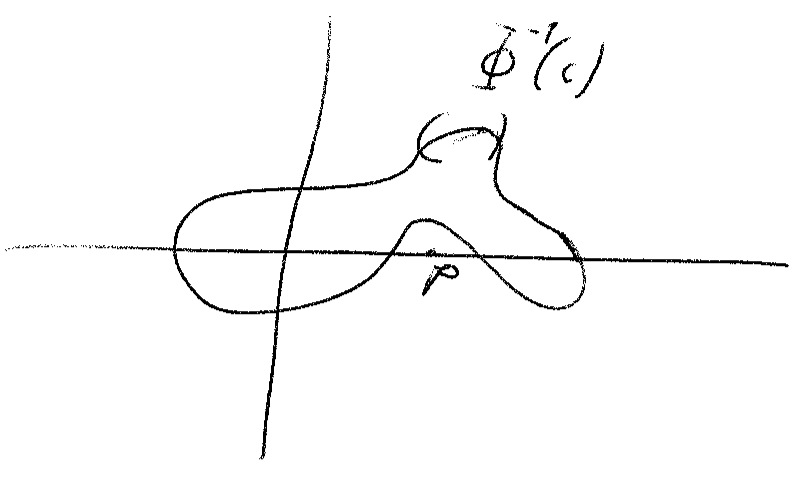
\includegraphics[width=.7\textwidth]{sketch_2_02.png}
        \caption{Sketch 2.02}
    \end{figure}

    Let \(M=\phi^{-1}(c)\). We define \(\hat{\pi_i}:\R^{n+1}\to\R^n,(x_0,\dots,x_n)\mapsto (x_0,\dots,\hat{x_i},\dots,x_n)\).
    \[\{(U,\hat{\pi_i})\mid U\subset M, \hat{\pi_i}\mid_U\text{ homeomorphism, } \partial_{x_i}\Phi\neq 0\text{ on } U\}\]

    Remains to check the formula:
    \[\hat{\pi_j}\circ \hat{\pi_i}^{-1}(y_1,\dots,y_n)=\begin{cases}
        (y_1,\dots,f,\dots,\hat{y_j},\dots,y_n)& j>i\\
        (y_1,\dots,\hat{y_{j+1}},\dots,f,\dots, y_n)& i<j\\
        (y_1,\dots,y_n) & i=j 
    \end{cases}\]
\end{example}

\begin{remark}
    The condition \(D\Phi\neq 0\) is very explicit! It is very easy to generate lots of manifolds. For example: \(\Phi(x)=\sum \lambda_i x_i^2\)
\end{remark}

\begin{example}[Example 5: Subset of smooth manifold] Let \(M\) be a smooth manifold. Then 
     \(U\subset M\) open, is also a smooth manifold. (Take charts of \(M\) and intersect / restrict each chart)
\end{example}

\begin{example}[Example 6: Product of manifolds] Let \(M,N\) be smooth manifolds. Then \(M\times N\) is also a 
    smooth manifolds. Take as charts \marginnote{This takes care of the torus!}
    \[\{(U\times V, (\phi,\psi))\mid (U,\phi),(V,\psi)\text{ charts of M,N respectively}\}\]
\end{example}

\begin{example}[Example 7: ]\marginnote{This is one to pay \dhighlight{attention} to!}
    Let's consider \(\R\). We define a chart \(\R\to\R,x\mapsto x^3\). Observe that 
    \[M=(U=\R,U\stackrel{\text{id}}{\to}\R)\]
    and 
    \[N=(U=\R,U\stackrel{x\mapsto x^3}{\to}\R)\]
    are smooth manifolds, which are different! Since the transition functions between them are not smooth:

    Indeed \(\text{id}\circ (x\mapsto x^3)^{-1}=(x\mapsto x^{\frac{1}{3}})\), which is not smooth!
\end{example}

\subsection{Smooth maps}

\begin{definition*}
    Let \(M\) be a smooth manifold. A map \(f:M\to\R^m\) is said to be \dhighlight{smooth}, if for all 
    \(p\in M\), there exists a chart \((U,\phi)\) containing \(p\), such that
    \[f\circ \phi^{-1}:\underbrace{\phi(U)}_{\subset\R^n}\to\R^m\] 
    is smooth. 
\end{definition*}

\begin{definition*}\marginnote{manifolds \(=\) smooth manifolds as always (unless otherwise stated)}
    Let \(M,N\) be manifolds. We say \(f:M\to N\) is \dhighlight{smooth} if, for all \(p\in M\) 
    there exists charts \((U,\phi)\) with \(p\in U\subset M\) and \((V,\psi)\) with \(V\subset N\) such that: 
    \begin{itemize}
        \item \(V\supset f(U)\)
        \item \(\psi\circ f\circ \phi^{-1}:\underbrace{\phi(U)}_{\subset\R^n}\to\R^m\) is smooth
    \end{itemize}
\end{definition*}

Reality check.

\begin{lemma}
    Smooth maps are continuous.
\end{lemma}

\begin{proof}
    Enough to show that \(\forall p\in M\), there exists a neighborhood of \(p\) on which \(f:M\to N\) is 
    continuous, for \(f\) smooth. By definition \(\exists (U,\phi),p\in U,(V,\psi),V\subset N\) s.t. 
    \(\psi \circ f\circ \phi^{-1}:\phi(U)\to\R^m\) smooth.

    Observe \(f=\psi^{-1}\circ (\psi \circ f\circ \phi^{-1})\circ \phi\) on \(U\).
\end{proof}

\begin{lemma}
    \(f:M\to N\) is smooth if and only if each \(p\in M\) has a neighborhood \(U\) suhc that \(f\mid_U\) is smooth.
\end{lemma}

\begin{proof}
    Sheet 03.
\end{proof}

\begin{lemma}[Properties of smooth maps]
    \begin{enumerate}
        \item[(i)] Any constant map \(c:M\to N\) is smooth\footnote{Since it sends \(M\) to a point in \(N\)}
        \item[(ii)] The identity map \(\text{id}:M\to M\) is smooth 
        \item[(iii)] If \(U \circ M\) open, then the inclusion \(i:U\hookrightarrow  M\) is smooth
        \item[(iv)] Compositions of smooth functions are smooth
    \end{enumerate}
\end{lemma}

\begin{proof}
    Sheet 03.
\end{proof}

\begin{definition*}\marginnote{In particular, diffeomorphisms are homeomorphism!}
    Let \(M,N\) be manifolds. A \dhighlight{diffeomorphism} \(f:M\to N\) is a smooth 
    map, which is bijective and admits a smooth inverse.
\end{definition*}

\begin{example}
    \(f:\R\to\R,x\mapsto x+3\) is a diffeomorphism with inverse \(x\mapsto x-3\).  
\end{example}

\begin{example}
    Let \(A\in\text{GL}(n,\R)\). Define a map \[f_A:\R^n\to\R^n,x\mapsto Ax.\]
    This is a diffeomorphism (smooth, since linear) with inverse \(f_A^{-1}=f_{A^{-1}}\).  
\end{example}

\begin{example}
    Let \(S_c^n\coloneqq \{(x_0,\dots,x_n)\mid \sum_{i=0}^n x_i^2=c^2\}\subset\R^{n+1}\). Given 
    \(d>c>0\), we define a diffeomorphism. 
    \[S_c^n\to S_d^n, (x_0,\dots,x_n)\mapsto \frac{d}{c}(x_0,\dots,x_n).\]
\end{example}

\begin{example}
    \(M=(\R,\text{id}),N=(\R,x\mapsto x^3)\). The map \(M\to N, x\mapsto x^{\frac{1}{3}}\)
    is a diffeomorphism. Indeed, 
    \begin{align*}
        (x\mapsto x^3)\circ (x\mapsto x^{\frac{1}{3}}) \circ\text{id}^{-1}=\text{id}
    \end{align*}
\end{example}

\subsection{The category of smooth manifolds}

\begin{definition*}
    Let \(\text{Man}^\infty\) be the category of smooth manifolds. The objects are the smooth manifolds. 
    The morphisms are the smooth maps.
\end{definition*}

\dhighlight{Exercise}: \(M,N\) objects in \(\text{Man}^\infty\) are isomorphic if and only if they are diffeomorphic.

Observe that there is a forgetful functor: \(\maninf\to\man0\) by \( (M,[\cA])\to M\) and \(f:M\to N\mapsto f\).

In general:\begin{itemize}
    \item not full 
    \item not essentially surjective
\end{itemize}

\begin{remark}[Hierarchy of categories]
    \begin{itemize}
        \item for \(k=0,\dots,\infty\), we can consider the category \(\mank\) with objects \(C^k\)-Manifolds, and morphisms \(C^k\)-maps. 
              for \(k\leq l\) there is a forgetful functor \(\text{Man}^l\to\mank\)
        \item if \(k\geq 1\),then the forgetful functor \(\maninf\to\mank\) is essentially surjective. This is different from the \(C^0\) case. For this reason, we mainly focus on \(\man0,\maninf\). This is a theorem by Whitney
        \item there are other interesting categories: \(\text{Man}^{\text{Real-analytic}},\text{Man}^{\text{Cplx-analytic}},\dots\), which both come with a forgetful functor to \(\maninf\)
    \end{itemize}
\end{remark}

\begin{remark}[Classification of manifolds (not examinable)]
    \begin{itemize}
        \item all topological manifolds of dimension \(\leq 3\) admit a unique smooth structure
        \item \(S^7\), as a topological manifold, admits 15 pairwise non-diffeomorphic smooth structures. These are called \dhighlight{exotic spheres}. They also exist 
            in higher dimensions (Milan-Kervaire?)
        \item \(\R^4\) admits uncountably many pairwise non-diffeomorphic smooth structures (Taubes~1980s)
        \item Open problem(\dhighlight{Smooth 4 dimensional Poincaré conjecture}): Prove or disprove: any smooth 
              4-manifold, which is homeomorphic to \(S^4\) is diffeomorphic to \(S^4\). Most experts believe this is false!  
    \end{itemize}
\end{remark}

\beginlecture{05}{22.10.2024}

\subsection{Smooth manifolds with boundary} % TODO: Wrong number?

\begin{definition*}
    A function \(f:\bH^n\supset U \to \R^k\) is \dhighlight{smooth} if every \(p\in U\)
    admits an open neighborhood \(p\in U_p\subset\R^n\) on which \(f\) extends to a smooth function. (i.e. there exists \(\tilde{f}_p:U_p\to\R^k,\tilde{f}_p\) smooth and \(\tilde{f}_p\mid_{\bH^n\cap U}=f\))
\end{definition*}

\begin{example}
    \(n=1,\bH^1=[0,\infty), f(x)=x^2\)
\end{example}
\begin{example}[Non-Example]
    \(n=1,\bH^1=[0,\infty), f(x)=\sqrt{x}\) has no smooth extension to \(0\), since the derivative goes to \(\infty\).
\end{example}

Give a topological manifold with boundary, we can define unproblematically the notions of 
\begin{itemize}
    \item smoothly compatible charts: \((U,\phi):M\to\bH^n\), \(\phi_\alpha\circ \phi_\beta^{-1}:\phi_\beta(U_\alpha\cap u_\beta)\to\bH^n\)
    \item smooth atlases
\end{itemize}

\begin{definition*}
    A smooth manifold with boundary \(M=(M,[\cA])\) is the data of 
    \begin{itemize}
        \item a topological manifold with boundary 
        \item an equivalence class of atlases 
    \end{itemize}    
\end{definition*}

\begin{remark}\marginnote{Similarly we cna generalise even more to manifolds with corners ...}
    Every smooth manifold is a smooth manifold with boundary. This is an enlargement of 
    \(\maninf\).
\end{remark}

\section{Partitions of unity}\marginnote{This section is technical, but also very important!}

\subsection{Preparatory lemmas}

\begin{lemma}\label{lem:2.4}
    The function \(f:\R\to\R,\)
    \[f(t)=\begin{cases}
        e^{-\frac{1}{t}} & t>0\\
        0 & t\leq 0
    \end{cases}\]
\end{lemma}

\begin{proof}
    It is enough to proof, that \(f\) has well defined derivatives of all orders, since \(f\) is a function on \(\R\).

    \(f^0=f\), for  \(k\geq 1\), assume \begin{enumerate}
        \item \(f^{(k-1)}\) exists
        \item \(f^{(k-1)}\mid_{(-\infty,0]}=0\) 
        \item \(f^{(k-1)}\mid_{(-\infty,0]}(t)=P_{k-1}(\frac{1}{t})e^{-\frac{1}{t}}\) for some polynomial \(P_{(k-1)}\).
    \end{enumerate}
    Clearly this holds for \(k=1\). 
    
    We have \begin{align*}
        \lim_{t\to0^+}\frac{f^{(k-1)}(t)-f^{(k-1)}(0)}{t}&=\lim_{t\to 0^+}\frac{f^{(k-1)}(t)}{t}\\
        &=\lim_{t\to 0^+}P_{(k-1)}(\frac{1}{t})\frac{1}{t}e^{-\frac{1}{t}}\\
        &= \lim_{x\to\infty} P_{(k-1)}(x)\cdot x\cdot e^{-x}=0
    \end{align*}
    Therefore \(f^{(k-1)}\) is differentiable at the origin, the derivative \(f^{(k-1)'}(0)=0\).
    and \(f^{(k-1)}\mid_{(-\infty,0]}=0\). Therefore \(f^{(k-1)}\) is differentiable.
    Therefore we only have to check 3., which only takes place on \(\R_+\)! 

    Finally \(f^{(k-1)}\mid_{(0,\infty)}(t)=P_{(k-1)}(\frac{1}{t})e^{-\frac{1}{t}}\implies P_{(k-1)}'(\frac{1}{t})\left(\frac{-1}{t^2}e^{-\frac{1}{t}}+P_{(k-1)}(\frac{1}{t})e^{-\frac{1}{t}}\right)\eqqcolon P_{(k)}(\frac{1}{t})e^{-\frac{1}{t}}\).
\end{proof}

\begin{lemma}\label{lem:2.5}
   Fix real numbers \(r_1<r_2\). Then there exists a smooth function \(h:\R\to\R\) such that 
   \begin{enumerate}
    \item \(h=1\) on\((-\infty,r_1]\)
    \item\(0<h<1\) on \(r_1,r_2\)
    \item \(h=0\) on \([r_2,\infty)\)
    \end{enumerate}
\end{lemma}

\begin{proof}
    \(h(t)\coloneqq \frac{f(s_2-t)}{f(s_2-t)+f(t-s_1)}\), since the denominator never goes to \(0\).
\end{proof}

\begin{lemma}[Existence of \dhighlight{cutoff functions}]\label{lem:2.6}
    Given \(0<r_1<r_2\), there exists a smooth function \(H:\R^n\to\R\) such that 
    \begin{enumerate}
        \item \(H=1\) on \(\overline{B_{r_1}}\)
        \item \(0<H<1\) on \(B_{r_2}\setminus \overline{B_{r_1}}\)
        \item \(H=0\) on \(\R^n\setminus B_{r_2}\)
    \end{enumerate}
\end{lemma}

\begin{proof}
    Set \(H(x)\coloneqq h(|x|)\), where \(h\) is defined as in lemma \ref{lem:2.5}. (Recall: \(|x|\coloneqq \sqrt{x_1^2+\dots+x_n^2}\)).
    Then \(H\) is smooth, since it is a composition of smooth functions on \(\R^n\setminus \overline{B_{r_1}}\) and constant on \(\overline{B_{r_1}}\).
\end{proof}

\subsection{Partitions of unity}

\begin{definition*}
    Given a topological space \(X\) and a function \(f:X\to\R\), the \dhighlight{support} of \(f\) is the set 
    \[\supp(f)\coloneqq\overline{ \{x\in X\mid f(x)\neq 0\}}\subset X\]
\end{definition*}

\begin{example}
    If \(f:\R\to\R\) has the form \(f(x)=a_0+a_1x+\dots,a_nx^n\implies \supp(f)=\R\).
    In fact, by Taylor's theorem, if \(f\) analytic, then \(\supp(f)\) either \(\R\) or \(\emptyset\).
    In contrast, the function \(h:\R\to\R\) defined in lemma \ref{lem:2.5} has support \((-\infty,r_2]\subsetneqq\R\).
\end{example}

% TODO: Fix = to ---

\begin{definition*}
    Let \(M\) be a smooth manifold. Let \(\{U_\alpha\}_{\alpha\in \cA}\) be an open cover. 
    A \dhighlight{partition of unity subordinate to the cover} is the data of a collection of smooth functions \(\{\psi_\alpha\}_{\alpha\in\cA},\psi_\alpha:M\to\R\)
    such that 
    \begin{enumerate}
        \item[(1)] \(0<\psi_\alpha<1\)
        \item[(2)] \(\supp(\psi_\alpha)\subset U_\alpha\)
        \item[(3)] \(\{\supp(\psi_\alpha)\}_{\alpha\in\cA}\) is locally finite 
        \item[(4)] \(\sum_{\alpha\in\cA} \psi_\alpha=1\)    
    \end{enumerate}
\end{definition*}

\begin{remark}
    There is an analogous notion in the category Top,\(\man0,\mank\), etc.,\dots
\end{remark}

\begin{example}
    \(M=\R\), \(U_1=(-\infty,r_2+1),U_2=(r_1-1,\infty)\), where \(r_1<r_2\) as in lemma \ref{lem:2.5}.
    Similarly let \(h\) as in lemma \ref{lem:2.5}. and set \(\psi_1=h,\psi_2=1-h\)
\end{example}

\begin{theorem}[Existence of partitions of unity]\label{thm:2.7}
    Let \(M\) be a smooth manifold. Let \(\{U_{\alpha}\}_{\alpha\in\cA}\) be an open cover. 
    Then there exists a partition of unity subordinate to this cover. 
\end{theorem}

\begin{remark}
    The same theorem works in Top, \(\man0,\mank\). It will not work in \(\text{Man}^{\text{Analytic}},\text{Man}^{\text{Cplx-Analytic}},\) Varieties \(/\C\).
\end{remark}

\begin{proof}
    \dhighlight{Step 1: Construction of the \(V_i\)} An open supset \(U\subset M\) is called a \dhighlight{regular coordinate ball} if there 
    exists \(\overline{U}\subset\tilde{U},(\tilde{U},\tilde{\phi})\) a chart such that 
    \(\tilde{\phi}(U)=B_{r_1},\tilde{\phi}(\tilde{U})=B_{r_2}\). 
    % skecth 2.06

    By lemma \ref{lem:1.6} \(M\) admits an exhaustion by compact sets. By lemma \ref{lem:1.7}, given 
    any basis, any open cover, one can find a locally finite, countable basis refinement of this cover by basis elements.

    Claim: \(\{\text{regular coordinate balls}\}\) basis of \(M\) \marginnote{The claim is easy to verify}

    These tree points imply that \(\{U_\alpha\}_{\alpha\in\cA}\) admits a countable, locally finite refinement by regular coordinate balls \(\{V_i\}_{i\in I}\).

    By sheet 2, exercise 1 (a) \(\{\overline{V_i}\}\) is still locally finite.

    \dhighlight{Step 2: Construction of the \(f_i\)} For each \(V_i\exists V_i\supset \tilde{V_i},\tilde{\phi_i}:\tilde{V_i}\to \R^n\) such that 
    \(\tilde{\psi_i}(V_i)=B_{s_1^i},\tilde{\psi_i}(\tilde{V_i})=B_{s_2^i}\) with \(0<r_1^i<r_2^i\), \(\tilde{V_i}\subset U_\alpha\) for some \(\alpha\).
    Using lemma \ref{lem:2.6}, let \(H_i:\R^n\to \R\) be a cutoff function, i.e. \(H_i\mid_{{B_{r_1}}}>0,H=0\) on \(\R\setminus B_{s_1^i}\).

    Let us set \(f_i:M\to\R, f_i=\begin{cases}
        H_i\circ \tilde{\phi_i} & \text{ on } \tilde{V_i}\\
        0 & M\setminus \overline{{V_i}}
    \end{cases}\)

    \dhighlight{Step 3: Construction of the \(g_i\)} Let us set \(f=\sum_{i\in I} f_i\). This is well defined by local finiteness of the \(\overline{V_i}\) Note also that \(f>0\)..
    We set \(g_i=f_i/f\). Then clearly we have \(0\leq g_i\leq 1, \sum_{i\in I} g_i=1\)

    \dhighlight{Step 4: Reindexing and conformation} Since \(\tilde{V_i}\subset U_\alpha\), for some \(\alpha\), we can choose for each \(i\in I, \alpha(i)\in \cA\) s.t. \(V_i\in U_{\alpha(i)}\).
    Let us set \marginnote{Here the empty sum is \(0\)}\[\psi_{\alpha}\coloneqq \sum_{i\mid \alpha=\alpha(i)}g_i\]
    Observe for \dhighlight{(2)}: \[\supp(\psi_\alpha)=\overline{\bigcup_{\alpha(i)=\alpha} V_i}\stackrel{\text{Exercise 2.1}}{=}\bigcup_{\alpha(i)\alpha}\overline{V_i}\subset U_\alpha\]
    We still have \(0\leq \psi_\alpha\leq 1\), which is \dhighlight{(1)}
    
    and 
    \(\supp(\psi_\alpha)\) are locally finite: for each \(op\in M\), since \(\{\overline{V_i}\}\) locally finite,
    there exists a neighborhood \(U_p\) of \(p\)  which only intersects finitely many of the \(\{\overline{V_i}\}\), call 
    them \(V_1,\dots,V_k\). Then the only \(\psi_\alpha\) which have a chance of being non-zero must satisfy \(\alpha\in\{\alpha(1),\dots,\alpha(k)\}\) (this is \dhighlight{(3)}).

    Lastly \[\sum_{\alpha\in\cA}\psi_\alpha=\sum_{\alpha}\left(\sum_{i: \alpha=\alpha(i)} g_i\right)=\sum_{i\in I} g_i=1,\]
    which confirms \dhighlight{(4)}.

\end{proof}
\chapter{Tangent Vectors}

\section{Motivation}

Consider the following pictures 
\begin{figure}[H]
    \centering
    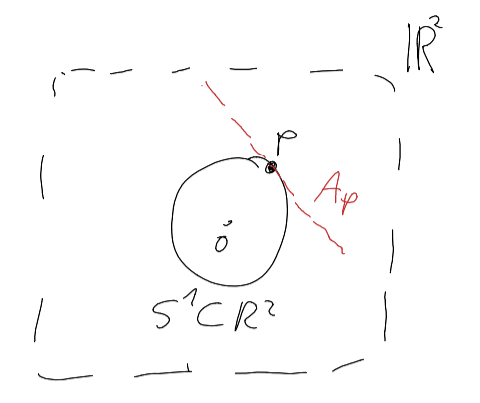
\includegraphics[width=.7\textwidth]{sketch_3_01.png}
    \caption{Sketch 3.01}
\end{figure}
\begin{figure}[H]
    \centering
    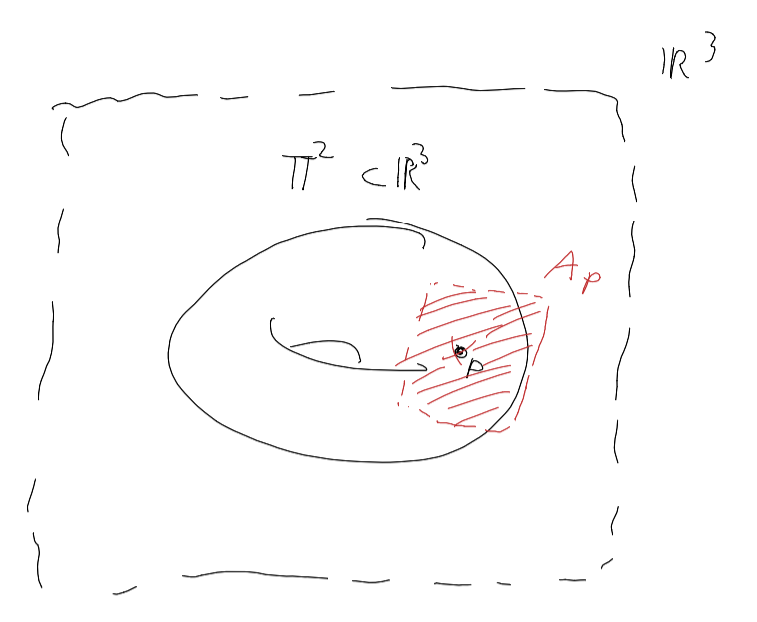
\includegraphics[width=.7\textwidth]{sketch_3_02.png}
    \caption{Sketch 3.02}
\end{figure}
\(A_p\) the affine hyperplane tangent to \(S^1 (\Pi^2)\) at the point \(p\).
Let \(T_p M\coloneqq A_p-p\subset\R^{n+1}\). This is a vector subspace of \(\R^{n+1}\).
It is called the \dhighlight{tangent space of \(M\) at \(p\)}. Consider \[TM=\bigcup_{p\in M} T_pM,\]
called the \dhighlight{tangent bundle}. Observe that there is a map 
\marginnote{Think of \(\pi\) as a map of \(p,T_pM\)}
\[\pi:TM\to M\]
by 
\[x\in T_p M\mapsto p\]
the data \(TM\stackrel{\pi}{\to}\) forms a \dhighlight{vector bundle}.

\dhighlight{Problems with this approach:}

\begin{itemize}
    \item not very intrinsic (depends on \(R^{n+1}\)\dots) 
    \item need to prove that manifolds can always embedded into \(R^N\)
\end{itemize}

This is really the picture / intuition we should have, but we will construct it in a different way.

\section{Two (equivalent) theories of tangent vectors} 

\subsection{Definition via equivalence classes of smooth curves}
\marginnote{I could not quite make out what he called this chapter, so I named it according to 
\cite{taylor_equivalent}}

Let \(M\) be a smooth manifold. Fix \(p\in M\). 
\begin{definition*}
    The \dhighlight{tangent space} of \(M\) at \(p\) denoted by \dhighlight{\(T_pM\)} is 
    the set of equivalence classes of smooth curves \(gamma:[-\epsilon,\epsilon]\to M,\gamma(0)=p\)
    with \(\gamma_1\sim\gamma_2\iff\) for any smooth function \(f\) defined near\footnote{in a neighborhood of} \(p\), we have 
    \((f\circ\gamma_1)'(0)=(f\circ \gamma_2)'(0)\). Here the \(\epsilon>0\) is any positive real number, which depends on \(\gamma\).
\end{definition*} 
\begin{figure}[H]
    \centering
    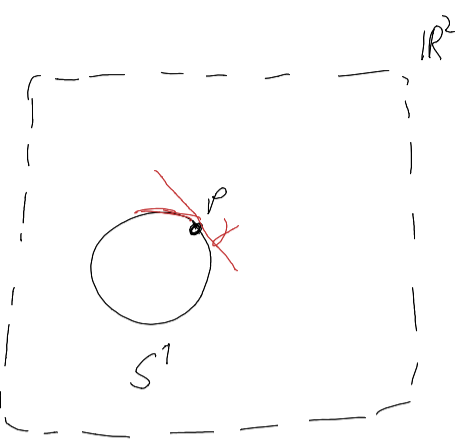
\includegraphics[width=.7\textwidth]{sketch_3_03.png}
    \caption{Sketch 3.03}
\end{figure}

\begin{definition*}
    Given a smooth map \(F:M\to N\), let
    \[dF_p:T_pM\to T_{F(p)}N\]
    be given by \marginnote{This is clearly well defined}
    \[[\gamma]\mapsto [F\circ\gamma].\]
    This map \(dF_p\) is called the \dhighlight{differential of \(F\) at \(p\)}.
\end{definition*}

\begin{remark}
    The map is also called the \dhighlight{tangent map of \(M\) at \(p\)} and the \dhighlight{total derivative}.
    It is also denoted by \[DF_p,TF_p,\nabla F_p,F_p',DF(p),TF(p),\dots\]
\end{remark}

\begin{lemma}[Fundamentality of the differential]\label{lem:3.1}
    Let \(F^1:M_1\to M_2\), \(F^2:M_2\to M_3\) smooth. Then:
    \begin{enumerate}
        \item[(i)]\(dF^2_{F^1(p)}\circ dF_p^1=d(F^2\circ F^1)_p\)
        \item[(ii)] If \(F:M\to M\) is he identity, then \(dF_p=\text{id}\)  
    \end{enumerate}
\end{lemma}

\begin{proof}
    Exercise.
\end{proof}
\chapter{Submersions, immersions and embeddings}

\section{Basic definitions}

\begin{definition*}
    Let \(F:M\to N\) be smooth. The \dhighlight{rank} of \(F\) at \(p\in M\)
    is the rank of the linear map \(dF_p:T_p M \to T_{F(p)}M\).
\end{definition*}

Smooth maps, which have full rank (highest possible rank, i.e. \(\text{rank} F=\max(m,n)\)) are particularly important:
\begin{definition*}
    Let \(F:M^m\to N^n\) be smooth. \marginnote{\(M^m,N^n\) means \(M,N\) are \(m,n\) dimensional manifolds}
    We say \begin{itemize}
        \item \(F\) is a \dhighlight{submersion} if \(dF_p\) is surjective, for all \(p\in M\) (\(m\geq n\))
        \item \(F\) is an \dhighlight{immersion} if \(dF_p\) is injective, for all \(p\in M\) (\(m\leq n\))
    \end{itemize}
\end{definition*}

\begin{lemma}\label{lem:4.1}
    Given \((m,n)\in \N_+\times \N_+\), let \(\Mat(m\times n)\equiv \R^{m\times n}\).
    The subset \(\Mat(m\times n)^{\text{full rank}}\coloneqq \{A\in \Mat(m\times n)\mid A\text{ has full rank}\}\)
    is open in \(\Mat(m\times n)\).
\end{lemma}

\begin{proof}
    Fix \(M\in\Mat(m\times n)^{\text{full rank}}\). Without loss of generality \(m\leq n\), otherwise 
    apply \(\Mat(m\times n)\to \Mat(n\times m),A\mapsto A^T\). By definition 
    there exists a submatrix \(M'\), obtained by deleting \(n-m\) columns, which is invertible.
    Now the map \marginnote{\(M\) is fixed and \(F\) depends on \(M\), but it does not matter here!}
    \begin{align*}
        f\Mat(m\times n)\stackrel{F:M\mapsto M'}{\to} \Mat m\times m\stackrel{\text{det}(\cdot)}{\to} \R
    \end{align*}
    is continuous, since booth the forgetful \(F\) and det is smooth.
     \[M\in (\det\circ F)^{-1}(\underbrace{\R\setminus\{0\}}_{\text{open}})\subset \Mat(m\times n)^{\text{full rank}}\]
    since \(M\) was arbitrary this completes the proof.
\end{proof}

\begin{lemma}\label{lem:4.2}\marginnote{The property of full rank is stable under small pertubation!}
    Fix \(F:M^m\to N^n,p\in M\).
    \begin{enumerate}
        \item If \(dF_p\) is injective, then there exists a neighborhood of \(p\) on which 
              \(dF_{\cdot}\) is injective. 
        \item If \(dF_p\) is surjective, then there exists a neighborhood of \(p\) on which 
        \(dF_{\cdot}\) is surjective. 
    \end{enumerate}
\end{lemma}

\begin{proof}
    This is a local statement. We can therefore assume that \(M,N\) are open subsets of \(\R^m,\R^n\) respectively.
    Then \[dF_{(\cdot)}:M\to \Mat(n\times m)\] 
    is smooth, hence continuous. By assumption \(dF_p\in \Mat(n\times m)^{\text{full rank}}\). But \(\Mat(n\times m)^{\text{full rank}}\), so 
    the preimage is open (by lemma \ref{lem:4.1}) and contains \(p\).
\end{proof}

\begin{remark}\marginnote{important: contains both a definition and a counterexample!}
    \begin{enumerate} % TOFIX
        \item If \(F:M\to N\) is both an immersion and a submersion, then we say that \(F\) is a \dhighlight{local diffeomorphism}. We will see (Rank theorem %TOFIX
        ) that \(F\) is a local diffeomorphism \(\iff\forall p\in M\exists p\in U: F\restrict{U}\) is a diffeomorphism.
        \item be warned. local diffeomorphism need not be global: \begin{align*}
            \R^2&\equiv \C\supset &S^1=\{|z|=1\}&\to S^1\\
            (x,y)&\mapsto x+iy& z&\mapsto z^2
        \end{align*}
    \end{enumerate}
\end{remark}

\begin{definition*}
    An immersion is an \dhighlight{embedding} if it is a homeomorphism onto its image 
    with the subspace topology.
\end{definition*}

\begin{example}
    \begin{figure}[H]
        \centering
        \includegraphics[width=.7\textwidth]{example-image}
        \caption{Sketch 4.01}
    \end{figure}
    Another example: \[S^n=\{(x_0,\dots,x_n)\in\R^{1+n}\mid\sum x_i^2=1\}\subset\R^{1+n}\]
    with \[i:S^n\hookrightarrow \R^{1+n}\]

    \dhighlight{Non-examples}
    \begin{figure}[H]
        \centering
        \includegraphics[width=.7\textwidth]{example-image}
        \caption{Sketch 4.02}
    \end{figure}
    parametrized by \[t\mapsto (\sin t,\sin 2t)\]
    and 
    \begin{align*}
        \R&\mapsto \R^2/\Z^2&=S^1\times S^1\\
        t&\mapsto (t,\alpha t) & \alpha \in\R\setminus \Q 
    \end{align*}
    Can show\footnote{not obvious, examable} that the image is dense. It is an immersion, but no a homeomorphism!
\end{example}









\chapter{Submanifolds}
\section{Basic definitions}

\begin{definition*}
    Let \(M\) be a topological manifolds. A subset \(S\subset M\) is a \dhighlight{topological submanifold},
    if \(S\) is a topological manifold with the subspace topology.
\end{definition*}

\begin{example}
    \(S^n=\{(x_0,\dots,x_n)\mid \sum x_i^2=1\}\subset\R^{1+n}\)
\end{example}
\begin{example}[Non-example]
    \(\{(x,y)\mid x=0\lor y=0\}\subset\R^2\), since this is not a manifold (see sheet 01).
\end{example}
\begin{definition*}
    Let \(M\) be a smooth manifold. A topological submanifold \(S\subset M\) is a \dhighlight{smooth submanifold}, if 
    it is equipped with a smooth structure, s.t. the embedding \(i:S\hookrightarrow M\) is smooth.   
\end{definition*}

\begin{example}
    If \(M\) is a smooth manifold and \(U\subset M\) open, then \(U\subset M\) is a smooth manifold.\marginnote{With the restricted smooth structure of \(M\)}
\end{example}

%examples should not be inside tcolorboxes?

\begin{remark}
    Some authors (including Lee's textbook) use the term \dhighlight{embedded submanifold} to distinguish 
    from \dhighlight{immersed submanifolds}. For use ``submanifolds''\(\equiv\)``embedded submanifold''.
\end{remark}  

\begin{lemma}\label{lem:5.1}
    Suppose that \(f:M\to N\) smooth embedding. Let \(S\coloneqq F(M)\subset N\). Then 
    \(S\) admits a unique smooth structure making it a smooth submanifold, with the property that 
    \(f\) is a diffeomorphism onto its image.
\end{lemma}

\begin{proof}
    By definition of \(f\) being an embedding, \(f\) is a homeomorphism onto it's image, with the subspace topology.
    \(\implies S\) is a topological manifold. 

    We define a smooth atlas on \(S\) by taking \(\{(f(U),\varphi\circ f^{-1})\}\), as \((U,\varphi)\) ranges over the set of charts 
    for \(M\).

    Clearly \(f\) is a diffeomorphism, since \(\varphi\circ f\circ f^{-1}\circ\psi^{-1}\), for \((U,\varphi),(V,\psi)\) smooth charts, this follows 
    from the fact that \((U,\varphi),(V,\psi)\) are smoothly compatible on \(M\).

    This is the only smooth at with the property that \(f\) is a diffeomorphism, if \(\cB\) is an other such atlas, then the fact 
    that \(f\) is a diffeomorphism for \((S,\cB)\iff (S,\cA)\) compatible.

    Finally
    \begin{figure}[H]
        \centering
        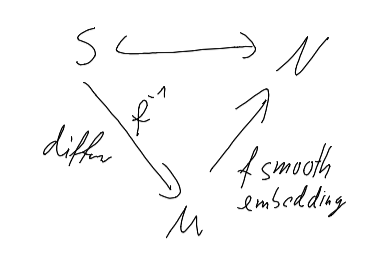
\includegraphics[width=.7\textwidth]{sketch_5_01.png}
        \caption{Sketch 5.01}
    \end{figure}
    so \(i\) is a smooth embedding.
\end{proof} 

\begin{definition*}
    A embedded submanifold \(S\) is called \dhighlight{properly embedded}, if the inclusion map 
    \(i\hookrightarrow N\) is proper (i.e. the preimage of a compact set is compact). 
\end{definition*}

\begin{example}
    \(S^n\hookrightarrow R^{n+1}\) properly embedded. 
\end{example}

\begin{example}[Non-example]
    \(S^n\setminus\{\text{pt}\}\subset\R^{n+1}\)
    \begin{figure}[H]
        \centering
        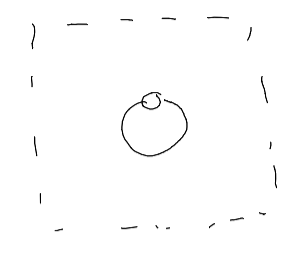
\includegraphics[width=.7\textwidth]{sketch_5_02.png}
        \caption{Sketch 5.02}
    \end{figure}
\end{example}

\begin{lemma}\label{lem:5.2}
    A topological submanifold \(S\subset N\) is properly embedded iff 
    \(S\) is closed.
\end{lemma}

\begin{proof}
    Exercise.\marginnote{Elementary exercise in point set topology}
\end{proof}

\section{The ``slice lemma''}

\begin{theorem}[Slice theorem]\label{thm:5.3}
    \begin{enumerate}
        \item[(a)] Suppose \(S^k\subset M^n\) is a Submanifold of codimension \(n-k\).\marginnote{this is also a definition of codimension: \(\dim M - \dim S\)}
                   Then, for all \(p\in S\), there exists a chart \((U,\varphi),p\in U\subset M\), such that \[\varphi(U\cap S)=\{(x_1,\dots,x_k,x_{k+1},\dots,x_n)\in \varphi(U)\mid x_{k+1}=c_{k+1},\dots,x_{n}=c_n\}.\]  
        \begin{figure}[H]
            \centering
            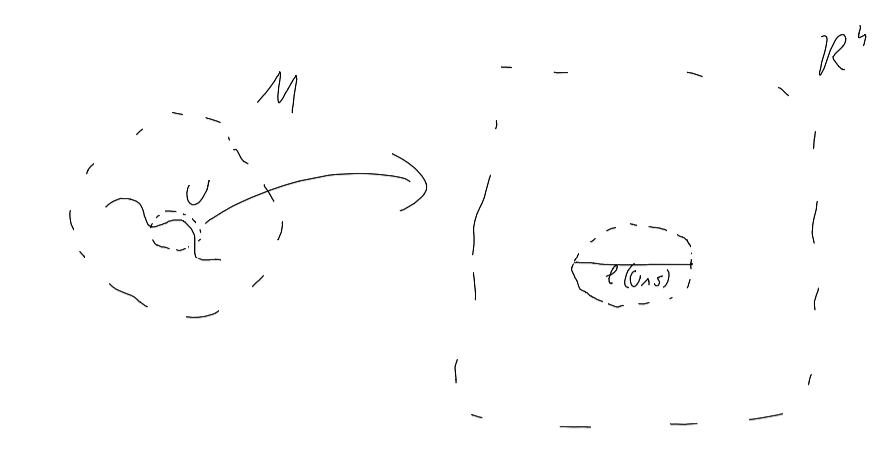
\includegraphics[width=.7\textwidth]{sketch_5_03.png}
            \caption{Sketch 5.03}
        \end{figure}
        \item[(b)] Done next time
    \end{enumerate}
\end{theorem}




\chapter*{Journal}
\addcontentsline{toc}{chapter}{Journal}
\begin{itemize}
    \renewcommand*{\do}[1]{\item \hyperlink{#1}{Lecture \StrBehind{#1}{c}:} Covering: \input{journal/#1}.\newline Starting in \Nameref{#1} and ending in \Nameref{#1end}. Spanning\pagedifference{#1}{#1end} pages}
    \dolistloop{\lecturelist}
\end{itemize}
\addcontentsline{toc}{chapter}{Bibliography}
\printbibliography
\end{document}